\documentclass[conference]{IEEEtran}
\IEEEoverridecommandlockouts

\usepackage[T1]{fontenc}
\usepackage[utf8]{inputenc}
\usepackage{cite}
\usepackage{amsmath,amssymb,amsfonts}
\usepackage{graphicx}
\usepackage{textcomp}
\usepackage{xcolor}
\usepackage{url}
\usepackage{booktabs}
\usepackage{array}
\usepackage{hyperref}
\usepackage{tikz}
\usetikzlibrary{arrows.meta,positioning}

\hypersetup{
  colorlinks=true,
  linkcolor=black,
  citecolor=black,
  urlcolor=blue
}

\begin{document}

\title{AI Risk Management and Continuous Data Protection\\
in Enterprise Generative-AI Systems}

\author{
\IEEEauthorblockN{Patrick Lemoine}
\IEEEauthorblockA{
\textit{Independent Researcher and Software Engineer}\\
Email: \texttt{lemoine\_patrick@yahoo.ca}\\
ORCID: \url{https://orcid.org/0009-0008-9465-8159}
}
}

\maketitle

\begin{abstract}
The rapid adoption of generative artificial intelligence (GenAI) has created a dual security challenge: organizations must manage immediate operational risks associated with data exposure, access control, hallucination, bias, and unapproved tool usage, while also preparing for emerging risks linked to autonomous agents, dual-use capabilities, and systemic dependencies. This paper argues that enterprise AI security cannot be reduced to model-level safety, because many high-impact failures originate in inadequate data classification, access control, retrieval governance, and workflow oversight. Enterprise AI security must therefore be implemented as a continuous governance and protection layer spanning data classification, identity and access management, prompt and output controls, private or enterprise-grade inference, auditability, and human oversight. We propose an event-driven architecture for intelligent Data Loss Prevention (DLP), in which semantic analysis, policy evaluation, and automated remediation operate on document lifecycle events. The proposed approach supports privacy-preserving deployment through local or private-cloud inference and aligns practical controls with contemporary risk-management frameworks, including the NIST AI Risk Management Framework, the European Union AI Act, and the OWASP Top 10 for Large Language Model Applications.
\end{abstract}

\begin{IEEEkeywords}
artificial intelligence, generative AI, large language models, AI governance, data loss prevention, data security, access control, zero trust, prompt injection, privacy, risk management
\end{IEEEkeywords}

\section{Introduction}

Generative AI systems based on large language models (LLMs) are increasingly used for document summarization, software development, knowledge retrieval, decision support, customer communication, and workflow automation. Their value derives from their ability to interpret unstructured information and generate contextually relevant outputs. However, this capability also expands the attack surface of the enterprise.

The public debate on AI safety often emphasizes long-term scenarios: superintelligent systems, autonomous self-improvement, loss of control, and alignment failures. These topics are scientifically and strategically relevant, but they should not obscure the operational risks that organizations face today. A confidential spreadsheet uploaded to an unapproved public AI service, a production credential embedded in a prompt, or an AI-generated response accepted without validation can cause immediate financial, legal, reputational, or security damage.

A central distinction is therefore required between \emph{data security} and \emph{model safety}. Data security concerns whether sensitive information is properly classified, protected, and accessible only to authorized actors. Model safety concerns whether an AI system behaves reliably, resists manipulation, respects policy constraints, and remains aligned with legitimate human objectives. Both dimensions are necessary, but they require different controls.

This paper presents a risk taxonomy for enterprise AI, identifies the principal security and governance requirements, and describes an event-driven architecture for continuous, AI-assisted data protection. The objective is not to propose unrestricted automation, but to define a practical control plane in which AI supports detection and classification while deterministic policies, identity controls, audit trails, and human review preserve accountability.

\section{Background and Motivation}

\subsection{From Periodic Audits to Continuous Governance}

Traditional data protection often relies on periodic audits, manual classification, static access-control reviews, and reactive incident response. These mechanisms remain necessary, but they are poorly suited to environments where thousands of documents are created, modified, shared, or processed every day.

Generative AI increases this pressure in several ways:

\begin{itemize}
  \item Employees can transfer sensitive content into external AI services through prompts, attachments, or retrieval workflows.
  \item AI agents may access enterprise systems through connectors, tools, and APIs.
  \item Retrieval-augmented generation (RAG) can expose documents that were not intended for a given user or context.
  \item Automated workflows may propagate incorrect or malicious content across systems.
  \item The boundary between user action, model inference, and downstream tool execution becomes increasingly diffuse.
\end{itemize}

Consequently, security must move from a periodic, document-centric model to a continuous, event-centric model.

\subsection{Regulatory and Framework Context}

Several contemporary frameworks reinforce this shift.

The NIST AI Risk Management Framework (AI RMF) provides a lifecycle-oriented approach organized around four functions: \emph{Govern}, \emph{Map}, \emph{Measure}, and \emph{Manage}. It is designed to help organizations incorporate trustworthiness considerations into the design, deployment, and evaluation of AI systems~\cite{nist_airmf}.

The European Union AI Act establishes a phased regulatory regime for AI systems and general-purpose AI (GPAI) models. Its general application began on 2 August 2026, although several obligations, particularly those applicable to high-risk AI systems, are subject to later implementation dates. Relevant requirements include transparency, documentation, risk management, traceability, and human oversight. High-risk AI systems face additional obligations, including risk assessment and mitigation, dataset quality, logging, documentation, and human oversight~\cite{eu_ai_act,eu_ai_act_timeline}.

The OWASP Top 10 for Large Language Model Applications identifies major security risks for LLM-based systems, including prompt injection, sensitive information disclosure, supply-chain vulnerabilities, data and model poisoning, improper output handling, excessive agency, system-prompt leakage, vector and embedding weaknesses, misinformation, and unbounded consumption~\cite{owasp_llm_top10,owasp_prompt_injection,owasp_llm_risks}.

These frameworks converge on a common principle: AI risk cannot be managed solely at the model layer. It must be governed across data, identity, application, infrastructure, and operational processes.

\section{Taxonomy of AI Risks}

\subsection{Immediate Operational Risks}

Immediate risks arise from the use of currently deployed models and AI-enabled workflows.

\subsubsection{Sensitive Data Disclosure}

Sensitive information may be disclosed when users submit confidential material to public AI services or when retrieval systems expose documents beyond the user's authorization boundary. Relevant data categories include personal data, health information, financial records, credentials, source code, contractual documents, trade secrets, and strategic plans. The OWASP LLM risk taxonomy explicitly identifies sensitive information disclosure as a major LLM application risk~\cite{owasp_llm_top10}.

\subsubsection{Prompt Injection and Indirect Instruction Manipulation}

Prompt injection occurs when adversarial input alters the intended behavior of an LLM. Direct injection may occur through user prompts, while indirect injection may occur through documents, emails, web pages, code repositories, or tool outputs processed by the model~\cite{owasp_prompt_injection}.

In enterprise settings, indirect prompt injection is particularly important because RAG pipelines and AI agents routinely process untrusted external content.

\subsubsection{Hallucination and Reliability}

LLMs can generate fluent but incorrect, incomplete, or misleading responses. In domains such as engineering, law, finance, healthcare, and scientific research, an unverified response may lead to erroneous decisions or unsafe actions.

Reliability controls should therefore include source attribution, confidence or uncertainty indicators where feasible, validation rules, and human review for consequential outputs.

\subsubsection{Bias and Discrimination}

AI systems trained or fine-tuned on historical data can reproduce or amplify social, cultural, or institutional biases. This is particularly sensitive in recruitment, credit scoring, insurance, healthcare, education, and judicial decision support.

Bias mitigation requires representative data governance, documented evaluation, fairness testing, and meaningful human oversight.

\subsubsection{Intellectual Property and Compliance}

Organizations must understand the provenance of training data, the contractual terms of AI services, and the conditions under which proprietary content may be submitted to external systems. The EU AI Act introduces transparency and copyright-related obligations for GPAI providers, including documentation and public summaries of training-content policies~\cite{eu_ai_act}.

\subsection{Systemic and Emerging Risks}

\subsubsection{Dual-Use Capability Amplification}

Advanced AI systems may lower the cost or expertise required to perform harmful tasks, including cyber reconnaissance, phishing, malware assistance, or the synthesis of dangerous chemical or biological knowledge. Defensive applications must therefore be balanced with access restrictions, usage monitoring, and model-level safeguards.

\subsubsection{Autonomous Agents and Excessive Agency}

AI agents can invoke tools, query databases, modify files, send communications, or execute code. The OWASP taxonomy identifies excessive agency as a key risk when an LLM system has more permissions, autonomy, or reach than necessary~\cite{owasp_llm_top10}.

The principle of least privilege must therefore apply not only to human users but also to AI agents and their tool invocations.

\subsubsection{Systemic Dependency}

As AI systems become embedded in finance, logistics, energy, telecommunications, healthcare, and public administration, localized failures may propagate through interconnected workflows. Cascading errors, degraded model behavior, corrupted retrieval indexes, or compromised connectors can produce effects beyond a single application.

\subsection{Long-Term Alignment Risks}

Long-term concerns include alignment, autonomy, self-improvement, and the possibility that highly capable systems could pursue objectives inconsistent with human intent. These questions require sustained research in interpretability, evaluation, corrigibility, oversight, and safe exploration.

However, organizations should not treat alignment as a substitute for present-day security. A practical AI risk program must address both horizons.

\section{Security of Data Versus Safety of Models}

\subsection{Data Security}

Data security concerns the protection of information throughout its lifecycle:

\begin{itemize}
  \item Classification
  \item Storage
  \item Access
  \item Transmission
  \item Processing
  \item Sharing
  \item Retention
  \item Deletion
\end{itemize}

If an AI assistant retrieves a confidential document that a user should not be authorized to access, the primary failure is often not the model itself. It may be a failure of classification, permissions, retrieval scoping, identity management, or policy enforcement.

\subsection{Model Safety}

Model safety concerns the behavior of the AI system:

\begin{itemize}
  \item Resistance to prompt injection
  \item Prevention of harmful or restricted outputs
  \item Reliability and factual grounding
  \item Resistance to jailbreaks and policy bypasses
  \item Control of tool usage
  \item Auditability of decisions and outputs
\end{itemize}

A secure enterprise AI system requires both dimensions. Strong model safeguards cannot compensate for excessive data permissions, and strong access controls cannot compensate for an AI system that can be manipulated into unsafe actions.

\section{Proposed Continuous AI-Assisted DLP Architecture}

\subsection{Architectural Principles}

The proposed architecture is based on five principles:

\begin{enumerate}
  \item \textbf{Event-driven monitoring}: security analysis is triggered by document and access events rather than scheduled scans alone.
  \item \textbf{Separation of concerns}: event capture, semantic analysis, policy evaluation, and remediation are decoupled.
  \item \textbf{Least privilege}: AI systems, agents, and retrieval components receive only the permissions required for their task.
  \item \textbf{Privacy-preserving inference}: sensitive content is analyzed in a trusted execution environment, private cloud, or on-premise deployment.
  \item \textbf{Human-in-the-loop}: automated actions are constrained by policy, confidence thresholds, auditability, and exception workflows.
\end{enumerate}

\subsection{High-Level Architecture}

Fig.~\ref{fig:architecture} illustrates the proposed architecture.

\begin{figure}[!t]
\centering
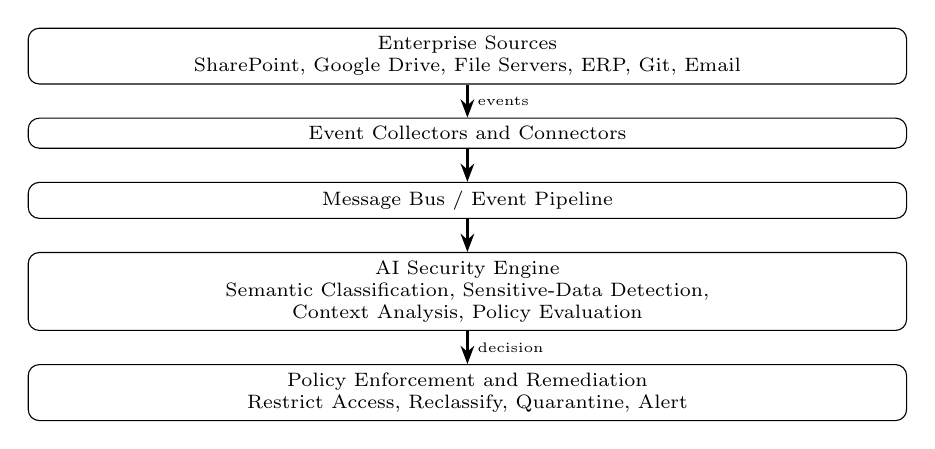
\begin{tikzpicture}[
  node distance=0.42cm,
  box/.style={
    draw,
    rounded corners,
    align=center,
    font=\scriptsize,
    inner sep=3pt,
    minimum width=0.92\columnwidth
  },
  arrow/.style={-{Stealth}, thick}
]

\node[box] (sources)
  {Enterprise Sources\\
   SharePoint, Google Drive, File Servers, ERP, Git, Email};

\node[box, below=of sources] (collectors)
  {Event Collectors and Connectors};

\node[box, below=of collectors] (bus)
  {Message Bus / Event Pipeline};

\node[box, below=of bus] (engine)
  {AI Security Engine\\
   Semantic Classification, Sensitive-Data Detection,\\
   Context Analysis, Policy Evaluation};

\node[box, below=of engine] (remediation)
  {Policy Enforcement and Remediation\\
   Restrict Access, Reclassify, Quarantine, Alert};

\draw[arrow] (sources) -- node[right, font=\tiny] {events} (collectors);
\draw[arrow] (collectors) -- (bus);
\draw[arrow] (bus) -- (engine);
\draw[arrow] (engine) -- node[right, font=\tiny] {decision} (remediation);

\end{tikzpicture}
\caption{Event-driven architecture for continuous AI-assisted DLP.}
\label{fig:architecture}
\end{figure}

\subsection{Component Description}

\subsubsection{Event Collectors}

Event collectors monitor document lifecycle actions such as creation, modification, renaming, movement, sharing, permission change, download, and external link generation. They emit lightweight events containing metadata such as event type, user identity, source system, file path, timestamp, and relevant content references.

\subsubsection{Message Bus}

A high-throughput message broker decouples event production from analysis and remediation. This enables horizontal scaling and prevents security analysis from directly blocking user-facing storage operations.

\subsubsection{AI Security Engine}

The AI Security Engine combines semantic and deterministic analysis:

\begin{itemize}
  \item \textbf{Semantic classification}: identifies the business or security domain of the content.
  \item \textbf{Sensitive-data detection}: identifies personal data, payment information, credentials, API keys, private keys, and other high-risk artifacts.
  \item \textbf{Context analysis}: evaluates consistency among content, storage location, classification label, recipient set, and intended use.
  \item \textbf{Policy evaluation}: applies organizational rules based on role, attribute, jurisdiction, data category, destination, and risk level.
\end{itemize}

A small language model (SLM) may be sufficient for many classification tasks when combined with deterministic detectors and rules. This is preferable to relying exclusively on a large general-purpose model, particularly for latency, cost, privacy, and auditability reasons.

\subsubsection{Policy and Access-Control Engine}

The policy engine evaluates whether the observed action is permitted. It should integrate:

\begin{itemize}
  \item Role-based access control (RBAC)
  \item Attribute-based access control (ABAC)
  \item Data classification labels
  \item Destination-folder policies
  \item External-sharing rules
  \item Jurisdictional and regulatory constraints
  \item Retrieval scoping rules
  \item Agent permission boundaries
\end{itemize}

\subsubsection{Remediation Module}

The remediation module executes approved actions through source-system APIs. Examples include applying a confidentiality label, restricting a public sharing link, revoking external access, moving a file to quarantine, blocking an AI retrieval request, sanitizing a prompt before external inference, generating a security alert, and creating an audit record.

\subsection{Example Workflow}

Consider an employee who saves a file named \texttt{Project\_Alpha\_Budget.xlsx} in a broadly shared marketing folder.

\begin{enumerate}
  \item The storage connector emits a \texttt{FILE\_CREATED} event.
  \item The event is published to the message bus.
  \item The AI Security Engine extracts and analyzes the document content.
  \item The system detects bank details, internal financial forecasts, and possibly credentials.
  \item The policy engine determines that the destination folder is not authorized for strictly confidential financial data.
  \item The remediation module restricts access, applies a confidentiality label, notifies the user, and alerts the security team.
  \item The event, decision, evidence, and remediation action are logged for audit purposes.
\end{enumerate}

This workflow transforms data protection from a retrospective audit into a near-real-time control process.

\section{Security Controls for LLM-Based Systems}

\subsection{Prompt and Output Protection}

LLM applications should implement controls on both input and output paths.

Input controls include prompt sanitization, detection of credentials, personally identifiable information, and proprietary code, classification of prompt sensitivity, restriction of external model usage for high-risk prompts, and detection of direct prompt injection.

Output controls include filtering sensitive data from responses, blocking unsafe tool invocations, enforcing output schemas for automated actions, logging generated content and tool calls, and applying human approval for high-impact actions.

These controls address several OWASP-identified risks, including prompt injection, sensitive information disclosure, improper output handling, and excessive agency~\cite{owasp_llm_top10}.

\subsection{Retrieval Security}

Retrieval-augmented generation systems require explicit retrieval governance:

\begin{itemize}
  \item Enforce per-user, per-role, and per-attribute retrieval filters.
  \item Apply document-level and chunk-level access control.
  \item Preserve provenance metadata through the retrieval pipeline.
  \item Prevent cross-tenant or cross-department contamination.
  \item Log retrieved sources and generated answers.
  \item Validate citations and source permissions.
\end{itemize}

A retrieval system must not become a mechanism that bypasses existing authorization rules.

\subsection{Agent Security}

AI agents require a dedicated permission model:

\begin{itemize}
  \item Define explicit tools and allowed operations.
  \item Apply least privilege to each tool.
  \item Require approval for irreversible actions.
  \item Separate read, write, administrative, and external-communication permissions.
  \item Limit execution scope, rate, budget, and blast radius.
  \item Maintain complete traces of prompts, tool calls, outputs, and decisions.
\end{itemize}

An agent should not receive broad system privileges merely because it can generate plausible natural-language instructions.

\subsection{Private and Enterprise Inference}

For sensitive workloads, organizations should evaluate enterprise AI services with contractual data-retention and no-training guarantees, private cloud endpoints, on-premise inference for highly sensitive content, local SLMs for classification and policy-support tasks, and hardware or software-based isolation where appropriate.

Open-source implementations can also support the exploration of privacy-preserving classification, sensitive-content detection, and policy-oriented analysis workflows~\cite{lemoine_llm_shield_scan}.

The choice depends on data sensitivity, latency requirements, compliance obligations, operational capacity, and total cost of ownership.

\section{Governance and Human Oversight}

\subsection{Governance Functions}

Following the NIST AI RMF, an enterprise program should establish governance structures that define accountability, risk tolerance, policies, roles, and lifecycle controls~\cite{nist_airmf}.

Key governance activities include maintaining an AI system inventory, defining acceptable-use policies, classifying AI use cases by risk level, assigning owners for data, models, applications, and agents, establishing incident-response procedures, conducting periodic risk assessments, monitoring model and system behavior, and reviewing third-party AI providers.

\subsection{Human-in-the-Loop}

Human oversight should be proportional to impact.

Low-risk tasks, such as grammar correction or internal summarization, may require minimal review. High-impact tasks---such as legal communication, financial decisions, security remediation, code deployment, or actions affecting individuals---should require explicit human approval.

Automation should assist decision-making, not remove accountability.

\subsection{Transparency and Documentation}

Organizations should document the purpose and scope of each AI system, data sources and retention rules, access-control model, evaluation and testing results, known limitations and failure modes, security controls, incident-response procedures, and human-review requirements.

This documentation supports internal governance, regulatory compliance, and operational resilience.

\section{Evaluation Metrics}

Table~\ref{tab:metrics} summarizes representative evaluation metrics for an AI-assisted DLP system.

\begin{table}[!t]
\caption{Evaluation Metrics for AI-Assisted DLP}
\label{tab:metrics}
\centering
\begin{tabular}{@{}p{0.30\columnwidth}p{0.62\columnwidth}@{}}
\toprule
\textbf{Category} & \textbf{Example metrics} \\
\midrule
Detection quality & Precision, recall, F1 score, false-positive rate, false-negative rate \\
Latency & End-to-end event-to-decision time, inference latency, remediation latency \\
Coverage & Monitored repositories, file types, sharing paths, and AI endpoints \\
Governance & Classified data assets, policy coverage, audit completeness \\
Security & Detected policy violations, blocked exposures, incident-response time \\
Usability & User override rate, false-alert burden, analyst workload \\
Privacy & Sensitive data sent to external services, private-inference coverage \\
\bottomrule
\end{tabular}
\end{table}

A system that produces excessive false positives will be bypassed by users. A system that produces too few alerts may create a false sense of security. The design objective is therefore calibrated protection, not maximal blocking.

\section{Limitations and Open Challenges}

\subsection{Semantic Ambiguity}

Natural-language understanding is probabilistic. A model may misclassify a document, fail to recognize context, or produce inconsistent labels across similar cases. Deterministic rules and human review remain necessary.

\subsection{False Positives and Operational Friction}

Overly aggressive blocking can reduce productivity and encourage users to circumvent controls. Deployment should begin in monitoring or advisory mode before enforcing restrictive actions.

\subsection{Privacy of the Security System}

An AI-based DLP system requires privileged access to sensitive content. It must therefore be protected as a high-value target, with strict access control, encryption, logging, isolation, vulnerability management, and independent auditability.

\subsection{Adversarial Adaptation}

Attackers may attempt to evade semantic detection through obfuscation, encoding, paraphrasing, or indirect injection. Security controls must therefore be layered and continuously evaluated.

\subsection{Agent Governance}

As agents gain the ability to plan and invoke tools, permission boundaries become more complex. Future work should explore formal capability constraints, verifiable tool policies, sandboxing, and runtime enforcement for agentic AI.

\section{Conclusion}

Enterprise AI security requires a broader perspective than model safety alone. Organizations must protect the data, identities, permissions, prompts, retrieval paths, tools, and workflows that surround generative-AI systems.

This paper has argued for a continuous, event-driven approach to AI-assisted data protection. By combining semantic analysis, sensitive-data detection, policy evaluation, least-privilege access control, private inference, auditability, and human oversight, organizations can reduce immediate data-exposure risks while preparing for more autonomous AI systems.

The proposed principles are also being explored through the open-source project LLM-SHIELD-SCAN~\cite{lemoine_llm_shield_scan}.

The strategic objective is not to build an all-powerful AI security model. It is to build a trustworthy control plane in which AI enhances detection and governance without weakening privacy, accountability, or human authority.

\section*{Acknowledgment}

The author acknowledges the growing open-source and industrial communities working on trustworthy AI, LLM security, data governance, and privacy-preserving machine learning.

\begin{thebibliography}{10}

\bibitem{nist_airmf}
National Institute of Standards and Technology,
``AI Risk Management Framework (AI RMF),''
NIST, Gaithersburg, MD, USA, 2026.
[Online]. Available:
\url{https://www.nist.gov/itl/ai-risk-management-framework}

\bibitem{eu_ai_act}
European Commission,
``AI Act,''
Shaping Europe's Digital Future, 2026.
[Online]. Available:
\url{https://digital-strategy.ec.europa.eu/en/policies/regulatory-framework-ai}

\bibitem{eu_ai_act_timeline}
Future of Life Institute,
``EU Artificial Intelligence Act: Implementation Timeline,''
Artificial Intelligence Act, 2026.
[Online]. Available:
\url{https://artificialintelligenceact.eu/implementation-timeline/}

\bibitem{owasp_llm_top10}
OWASP GenAI Security Project,
``OWASP Top 10 for Large Language Model Applications,''
OWASP Foundation, 2025.
[Online]. Available:
\url{https://owasp.org/projects/top-10-for-large-language-model-applications}

\bibitem{owasp_prompt_injection}
OWASP GenAI Security Project,
``LLM01:2025 Prompt Injection,''
OWASP Foundation, 2025.
[Online]. Available:
\url{https://genai.owasp.org/llmrisk/llm01-prompt-injection/}

\bibitem{owasp_llm_risks}
OWASP GenAI Security Project,
``LLM Risks Archive,''
OWASP Foundation, 2025.
[Online]. Available:
\url{https://genai.owasp.org/llm-top-10/}

\bibitem{lemoine_llm_shield_scan}
P. Lemoine,
``LLM-SHIELD-SCAN,''
GitHub repository, 2026.
[Online]. Available:
\url{https://github.com/lemoinep/LLM-SHIELD-SCAN}

\end{thebibliography}

\end{document}